\chapter{Occupancy Assessment}
\label{sec:occupancyAssessment}
Existing occupant sensing systems require the user to wear a
tag~\cite{smith2005rfid}, or to actively trigger a biometric sensor such as a
thumbprint or retina scanner~\cite{smith2005exploring}. These systems may be
practical in high security areas or some corporate office environments, but are
too inconvenient to use for residential applications such as HVAC control. Other
systems require cameras to be installed in the home that track
residents~\cite{nait4activity}. However, cameras are often perceived to be
invasive to personal privacy. Yet other systems require the installation of
smart floors~\cite{orr2000smart}, which incur a high initial cost and effort
that cannot be justified by applications such as Smart Zoning. With these
restrictions in mind, we leverage previous
research~\cite{srinivasan2008protecting,srinivasan2010using} that used cheap,
commercial off the shelf (COTS) motion sensors deployed in rooms and on doorways
in order to monitor room occupancy. We use a novel occupancy assessment
algorithm, described below, to detect occupancies needed to meet the
requirements of Smart Zoning as described in
Section~\ref{sec:occupancyAssessmentGoals}.

\section{Goals}
\label{sec:occupancyAssessmentGoals}

%% - Detect when rooms used

%% - Anecdote example of ``IDEAL''
%%  - Person starts using -> ``Occupied''
%%  - Stops               -> ``Unoccupied'' 

Smart Zoning aims to minimize energy wasted in conditioning rooms that are not
being used. Therefore, the goal of occupancy assessment is to detect when rooms
are used. In an ideal scenario, at night when two residents are asleep, only the
bedroom would be detected as being occupied. When one of the residents wakes up in
the morning and goes to the bathroom, the bathroom would be detected as being
occupied in addition to the bedroom. When the resident leaves the bathroom and
enters the kitchen, the bathroom would be detected as being unoccupied and the
kitchen would be detected as being occupied. Thus, the behavior desired, in the
ideal situation, is that of a room being used being detected as occupied, and
the moment the room stops being used, it being detected as unoccupied. 

%% - Find room usage with time constants commensurate with equipment operation

Such a room usage detection is ideal for the control of systems such as lights
or faucets where the required service is provided almost immediately when it is
activated and can be deactivated instantly when the service is not needed, with
no repercussions. An HVAC system, in contrast, takes time to heat or cool a
space, and therefore cannot react to occupants entering and leaving rooms
without sacrificing comfort and efficiency. Therefore, assessing room occupancy
goes beyond merely detecting when a room starts being used and stops being
used. The occupancy assessment algorithm for Smart Zoning has to find room usage
time constants commensurate with equipment operation periods. For instance, if
the HVAC system takes 15 minutes to heat the bathroom by one degree and the
resident enters and leaves the bathroom within a minute, detecting this
occupancy and reacting to it would waste energy while providing no benefit in
terms of comfort. Therefore, in assessing room occupancy, the system has to take
into consideration the HVAC equipment operation parameters.

%% - No short cycling -> Either damage -or- waste -or- discomfort | balance

Another issue that has to be considered when assessing occupancy is the short
cycling of HVAC equipment. Short cycling is the transition of the HVAC system
from an operating stage to a lower stage before the manufacturer recommended
minimum time. For instance, changing from stage 2 heat to stage 1 heat or
turning off from stage 1 cool before the minimum operating time for that
stage. Short cycling the HVAC system can cause equipment damage due to increased
wear and tear as a result of frequent equipment cycling and not allowing the
pressure within the system to equalize between cycles. 

In addition to potentially damaging hardware, short cycling could also waste
energy and subject the residents to discomfort. For instance, if a resident
spends most of his/her day in the living room but goes to the kitchen
periodically to get water or a snack, if the system did not consider short
cycling, the HVAC would turn off whenever the resident left the kitchen assuming
the living room was at the setpoint and the kitchen drifts away from the
setpoint due to being used infrequently. This turning on and off of the
equipment would waste energy while not providing any benefit to the
resident. Also, by allowing the kitchen to drift away from the setpoint, the
system would expended a large amount of energy in conditioning it when it is
used for a long period of time, such as when the resident is preparing a
meal. Similarly, short cycling the system would mean a room that is used
infrequently in conjunction with another room would never reach the setpoint
since the system turns off whenever the room stops being used. Thus, every time
the occupant enters the room s/he would be in discomfort. If occupancy
assessment only considered if a room was used or not in order to define it as
occupied or unoccupied, and actuated the HVAC system in response to this
information, short cycling would be inevitable. Thus, we need a more
sophisticated approach to occupancy assessment as will be described below. 

\section{Challenges}
\label{sec:occupancyAssessmentChallenges}

The challenges in assessing occupancy in most houses arise from room usage
durations not matching equipment operation periods and errors inherent in
sensing hardware. The mismatch in room usage durations and equipment operation
periods can manifest itself in {\em passageway rooms}, {\em multi-room usage},
 and {\em short-term room usage}. Inadequacies of hardware usually manifest
 themselves as false positives or negatives. In this section we describe these
 four challenges to occupancy assessment.

%% - Passageway rooms
\subsection{Passageway Rooms}
Passageway rooms are rooms, such as hallways, which connect two or more other
rooms. These could be central rooms in a house that are surrounded by other
rooms. Passageway rooms pose a challenge because they are constantly in use
throughout the day, yet for very short durations of time. Therefore, trading off
between saving energy and ensuring resident comfort becomes difficult. If
comfort was of utmost important passageway rooms would be considered as occupied
for most of the day so that whenever a resident passes through them they would
be at the comfortable setpoint temperature. Yet, because the amount of time a
resident spends in this rooms is a small fraction of a complete day, most of the
energy expended in maintaining the room at the setpoint would be
wasted. Thus, a successful occupancy assessment algorithm has to identify a room
as a passageway room so as not to waste energy conditioning when it is not
occupied, yet attempt to maintain it at close to the setpoint so that when
occupants pass through the room, as they are likely to do frequently throughout
the day, they are not discomforted. 

%% - Short-term usage
\subsection{Short-term Room Usage}

%% - Storage, bathroom, kitchen, wardrobe

In addition to passageway rooms, there are rooms that are usually not used for
long periods of time. For instance storage rooms, bathrooms, kitchens, and
wardrobes are entered for short periods of time throughout the day. These rooms
cannot be conditioned in response to usage because, in most instances, the rooms
are not occupied for a sufficient period of time for conditioning to be
effective. Differentiating short-term room usage from regular usage is a
challenge that has to be addressed in order to prevent the wastage of energy.

%% - Multi-room usage
\subsection{Multi-Room Usage}

%% Start/stop usage != enter/leave

There are many instances when rooms are used in groups. For instance a resident
may watch the news on television while preparing dinner, so that s/he alternates
between the kitchen and the living room, or set the dining table while keeping
an eye on a dish on the stove, alternating between the dining room and
kitchen. Such usage patterns cannot be identified and exploited if the occupancy
assessment algorithm defines room usage based on a resident entering and leaving
a room. In other words, a room does not necessarily start being used the moment
a person enters it and stop being used the moment the person leaves. The
occupancy assessment algorithm has to detect multiple rooms being used
concurrently so that they maybe conditioned as a group, increasing the
efficiency with which the HVAC system operates.

%% - Sensing false positive/negatives
\subsection{False Positives/Negatives}
\label{sec:falsePositives}

False positives and negatives are common errors associated with simple binary
occupancy sensors. PIR and X10 sensors can be triggered by shadows or the
changes in light levels due to the movement of the sun for instance resulting in
false positive sensor readings. These sensors also have a limited sensing radius
through which people have to move to be detected. Moving through blind spots
within a room can result in false negatives sensor readings. False positives
have to be overcome by filtering out spurious sensor firings while false
negatives have to be minimized by increasing the number of sensors in a room so
as to reduce the blind spots. Yet, these inadequacies of binary sensors have to
be considered when assessing occupancy.

\section{Approach}
\label{sec:occupancyAssessmentApproach}
%% - Learn room usage patterns

Our approach to occupancy assessment involves learning room usage patterns using
historical data and constantly evaluating the sensor firings to identify which
occupancy pattern a particular room that is in use is exhibiting. In order to
overcome the challenges described above we filter the raw sensor firings and
attempt to categorize occupied rooms as being either {\em transitionally
  occupied} or {\em stably occupied}. Ideally, passageway rooms, short-term room
usage, and initial room occupancy would be categorized as transitionally
occupied while rooms that are being used for longer periods of time, including
multi-room usage scenarios would be identified as stably occupied.   

%% - Model formulation
%% count/timeout 

The occupancy model used by Smart Zoning defines room usage based on rates of
sensor firings for transitional occupancy of stable occupancy to start or
end. Since the number of sensors differ per room, these rates of firing take the
sensor counts into consideration. Thus, for each room of the house, four sets of
parameters are defined in order to detect transitional occupancy or stable
occupancy starting or ending. Each set of parameters is composed of a firing
count, {\em C} and a timeout, {\em T}. For instance, for the living room to
start being transitionally occupied, the number of sensor fired within the
timeout defined for starting transitional occupancy divided by the number of
sensors in the room has to be greater than the firing count for the starting of
transitional occupancy. For transitional occupancy to end the number of sensors
fired within the timeout for transitional occupancy ending, normalized by the
number of sensors, should be less than the firing count for transitional
occupancy ending. Similarly, we use parameter to detect stable
occupancy. Transitional occupancies are usually based on shorter timeouts while
stable occupancies are based on longer timeouts.

%% - Optimization function 

The model is generated by processing historical occupancy data and searching for
parameters for each room using an optimization function. The process involves
three steps: (i) false positive minimization, (ii) search space generation, and
(iii) parameter selection which will be described below.

\subsection{False Positive Minimization}
As described in Section~\ref{sec:falsePositives} false positives occur when
sensors fire in a room that is not occupied. In order to minimize these
occurrences, which could lead to unoccupied rooms being assessed as occupied, we
aggregate sensor readings from multiple sensors in a room to filter out false
firings from any one sensor. As more sensors are aggregated, the possibility of
false positives occurring decreases. 

\begin{algorithm}                      % enter the algorithm environment
\caption{False Positive Minimization}          % give the algorithm a caption
\label{alg:fpFiltering}                           % and a label for \ref{} commands later in the document
\begin{algorithmic}                    % enter the algorithmic environment
\STATE $aggregateData = []$
\STATE $windowStartIndex = 1$
\WHILE{$windowStartIndex < length(sensorFirings)$}
\STATE $windowEndTime = sensorFirings(windowStartIndex) + oneMin$
\STATE $firingsBeforeEnd = sensorFirings < windowEndTime$
\STATE $firingsInWindow = firingsBeforeEnd(windowStartindex:end)$
\IF{$length(firingsInWindow) \geq numSensors / 2$}
\STATE $aggregateData.append(firingsInWindow(end))$
\STATE $windowStartInterval = windowEndInterval + 1$
\ELSE
\STATE $windowStartInterval = windowStartInterval + 1$
\ENDIF
\ENDWHILE
\end{algorithmic}
\end{algorithm}

Algorithm~\ref{alg:fpFiltering} describes the false positive filtering algorithm
Smart Zone utilizes. The filtering algorithm searches for one minute intervals
when the number of sensor firings for a particular room is at least half the
number of sensors in that room. Each time it finds such an interval, all the
sensor firings within that interval are aggregated into a single sensor
firings. by enforcing the requirement for at least half the sensors in a room to
fire, or a particular sensor fire at least $n/2$ times for a room with $n$
sensors, the filtering algorithm attempts to minimize instances when a single
spurious sensor firing is considered an indication of occupancy. This technique
also helps minimize false negatives because for any one minute interval only
$n/2$ sensors have to fire for that whole interval to be considered as having
a sensor firing. Thus, residents don't have to constantly keep triggering
sensors in order for them to be detected as being present in a room.

\subsection{Search Space Generation}
The search space generation algorithm attempts to estimate, for a range of
firing counts and timeouts for start and end, false positive counts, total
duration of occupancy detected, the number of transitions between occupied and
unoccupied states, and the 25th percentile value for time intervals. The range
of firing counts and timeouts are different when searching for transitional
occupancy parameters as opposed to stable occupancy parameters with transitional
occupancy parameters being searched for with lower firings counts and shorter
duration timeouts as compared to stable occupancy.

\begin{algorithm}                      % enter the algorithm environment
\caption{Search Space Generation}          % give the algorithm a caption
\label{alg:paramGen}                           % and a label for \ref{} commands later in the document
\begin{algorithmic}                    % enter the algorithmic environment
\FOR{$occStartCnt = occStartCntRange$}
\FOR{$occStartTO = occStartTORange$}
\FOR{$occEndCnt = occEndCntRange$}
\FOR{$occEndTO = occEndTORange$}
\STATE $occupancyTS = []$
\FOR{$i = 1:length(aggregateData)$}
\IF{$aggregateData(i + occStartCnt) - aggregateData(i) \leq occStartTO$}
\STATE $occupancyTS.append([aggregateData(i+occStartCnt-1), 1])$
\ELSIF{$aggregateData(i + occEndCnt) - aggregateData(i) > occEndTO$}
\STATE $occupancyTS.append([aggregateData(i) +
  occEndTO, 0])$
\ENDIF
\ENDFOR
\STATE $transCnt = 0$
\STATE $occDuration = 0$
\STATE $coveredFirings = []$
\STATE $iData = 1$
\STATE $vacancyStartTime = NaN$
\STATE $offIntervals = []$
\IF{$occupancyTS(1, 2) == 1$}
\STATE $occupancyStartTime = occupancyTS(1, 1)$
\ELSE
\STATE $occupancyStartTime = 0$
\ENDIF
\FOR{$j = 2:length(occupancyTS)$}
\IF{$occupancyTS(j - 1, 2) == 0 \: \AND \: occupancyTS(j, 2) == 1$}
\STATE $occupancyStartTime = occupancyTS(j, 1)$
\STATE $transCnt += 1$
\IF{$vacancyStartTime \neq NaN$}
\STATE $offIntervals.append(occupancyStartTime - vacancyStartTime)$
\ENDIF
\ELSIF {$occupancyTS(j - 1, 2) == 1 \: \AND \: occupancyTS(j, 2) == 0$}
\STATE $transCnt += 1$
\STATE $occDuration = occDuration +
occupancyTS(j, 1) - occupancyStartTime$
\WHILE{$aggregateData(iData) \leq occupancyTS(j,
  1)$}
\IF{$aggregateData(iData) \geq occupancyStartTime \: \AND \: aggregateData(iData) < occupancyTS(j, 1)$}
\STATE
$coveredFirings.append(aggregateData(iData))$
\ENDIF
\ENDWHILE
\ENDIF
\STATE $FNCnt = length(aggregateData) - length(coveredFirings)$
\STATE $offInt25 = prctile(offIntervals, 25)$
\STATE $params.append([FNCnt, transCnt, offInt25, occDuration, ...$
\STATE $occStartCnt, occStartTO, occEndCnt, occEndTO])$
\ENDFOR
\ENDFOR
\ENDFOR
\ENDFOR
\ENDFOR
\end{algorithmic}
\end{algorithm}

Algorithm~\ref{alg:paramGen} describes the algorithm used to generate the search
space over which the optimization function, described in
Section~\ref{sec:paramExt} searches for parameters with which to build the
occupancy model. This algorithm loops over the four sets of parameters for
occupancy start and end firing counts and timeouts. It first identifies times
when occupancy would be sensed as having started and ended based on these
parameters by iterating over the aggregated sensor firings, output by
Algorithm~ref{alg:fpFiltering} and comparing the number of firings within
windows defined by the timeouts for occupancy start and end to the appropriate
firing counts. Next, it iterates over the identified timestamps for occupancy
start and end and calculates the number of transitions, total amount of time the
house is detected as being occupied, and the number of false negatives: the
number of aggregated sensor firings that are in time intervals not considered
occupied. These parameters are stored in a matrix along with the occupancy start
and end timeouts and firing counts to be used by the parameter selection
algorithm.

\subsection{Parameter Selection}
\label{sec:paramExt}

The final stage of building the occupancy model is optimizing over the search
space generated by Algorithm~\ref{alg:paramGen}. The algorithm first prunes the
search space using three parameters, the maximum number of false negatives,
$FN$, the maximum number of transitions between occupied and unoccupied states,
$K$, and the minimum period for which a room would be detected as unoccupied for
at least 25\% of all the times the room transitions from occupied to unoccupied
and back to occupied, $T_{25}$. These three values were defined as expected
average values over a day. For stable occupancy we used $FN = 30$, $K = 4$, and
$T_{25} = 30 min$ and for transitional occupancy we used $FN = 4$, $K = 30$, and
$T_{25} = 3 min$. These values were selected to address the issues described in
Section~\ref{sec:occupancyAssessmentGoals} and
Section~\ref{sec:occupancyAssessmentChallenges}. In order to minimize short
cycling, we defined a longer $T_{25}$ for stable occupancy and defined $K$ to be
small. With these restrictions, we increased $FN$ to allow the algorithm some
flexibility in selecting parameters. For transitional occupancy, false negatives
were a concern since the aim of transitional occupancy is to capture occupancy
in passageway rooms and during short-term room usage. Thus, we defined a very
low threshold for $FN$ and a high threshold for $K$ since there would be many
transitional occupancy events during a day. Finally, we defined a short duration
for $T_{25}$ in order to capture the short periods of time when passageway and
short-term rooms are in use. 

\begin{algorithm}                      % enter the algorithm environment
\caption{Parameter Selection}          % give the algorithm a caption
\label{alg:paramSelection}                           % and a label for \ref{} commands later in the document
\begin{algorithmic}                    % enter the algorithmic environment
\FOR{$i = 1:length(params)$}
\IF{$params(i, 1) / numDays < FN \: \AND \: params(i, 2) / numDays < K
  \: \AND \: params(i, 3) \geq T_{25}$}
\STATE $candidateParameters.append(params(i, :))$
\ENDIF 
\ENDFOR
\STATE $minOccupiedDurationIndex = find(min(candidateParameters(:, 4)))$
\STATE $selectedParameters.append(candidateParameters(minOccupiedDurationIndex, 5:end))$
\end{algorithmic}
\end{algorithm}

Algorithm~\ref{alg:paramSelection} describes the algorithm used to select the
parameters for the occupancy model. The first phase of the algorithm is pruning
the search space by eliminating parameters that don't provide average daily
values of $FN$, $K$, and $T_{25}$ below, or above, the appropriate
thresholds. After this step, the $candidateParameters$ are searched for
parameters which result in the minimum amount of time the house is assessed as
being occupied. This minimizes false negatives. The parameters obtained from
this step are used to define occupancy for a particular room in the model.

%------------------------------------------------------------------------------
% Figure 5
\begin{figure}[t]
\centering{
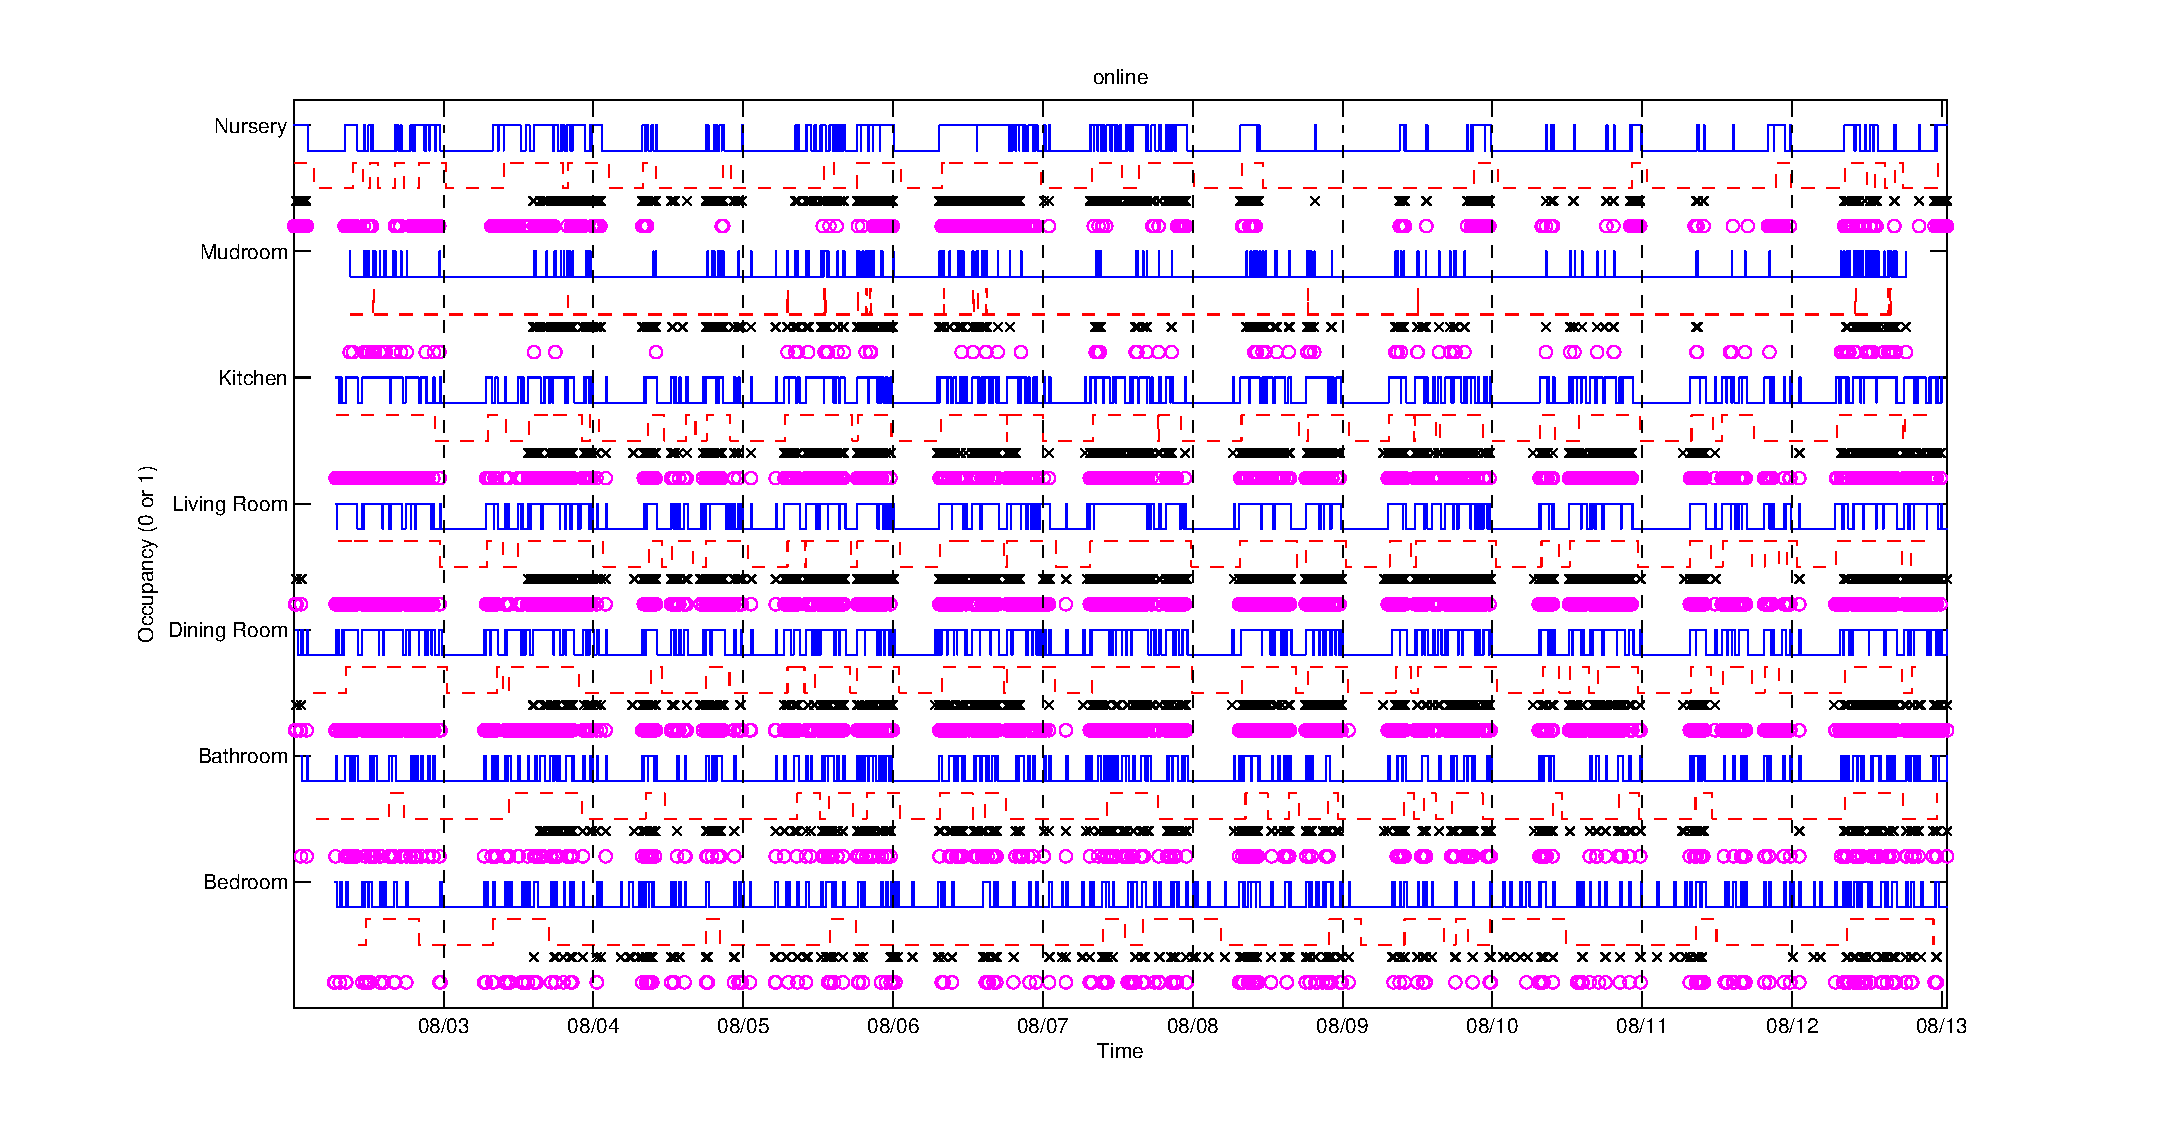
\includegraphics[width=1.0\columnwidth]{fig/occupancyTypes}
\caption[Transitional and Stable Occupancy Detected Using the Occupancy
  Model]{The solid line represents transitional occupancy, the dashed line
  represents stable occupancy, the X's depict the firings of the X10 motion
  sensors in rooms, and the O's depict the firings of the PIR sensors on
  doorways.}
\label{fig:occupancyType}}
\end{figure}
% ----------------------------------------------------------------------------

Using the parameters selected by Algorithm~\ref{alg:paramSelection} to process
sensor readings for a house over a period of ten days produces the occupancy
patterns as depicted in Figure~\ref{fig:occupancyType}. It is clear that
transitional occupancy captures frequent occupancy changes as detected by
aggregated sensor firings, while stable occupancy captures long-term room usage.


\section{Evaluation}

- Independent vars -> parameters and num sensors
- Metrics -> FN, short cycle, energy waste
- Comparison -> - reactive
                - uniform
                - whole house occupancy
